\par{The \emph{kernel} shown in listing \ref{private_memory_kernel} takes as a base the previous kernel, 
    but now it tries to use private memory to reuse a complete row of matrix A, this should bring a performance improvement
    due to the use of on chip memories in every of the devices studied, feature that neihter of the previous \emph{kernels}
    implemented.}

\lstinputlisting[float,caption={Kernel making use of \emph{private memory}.},label={private_memory_kernel}, 
                style=customc]{/Users/clalanne/GitHubProjects/OpenCLNotes/src/code/private_memory.c}

\par{Line \emph{9} of listing \ref{private_memory_kernel} shows the copy of elements of matrix A from \emph{global memory} to
    \emph{private memory}, this allows the reuse of that data to calculate several elements of matrix C without going to global
    again and again. One interesting issue that we can observed looking at the assembly code generated by the Xeon Phi, is that the 
    expensive gather operations from figure \ref{vtune_naive} in this \emph{kernel} became very cheap in comparison as it can
    be seen in figure \ref{vtune_rows} and also this figure shows that the \emph{vmovaps} \footnote{Moves packed single-precision 
    floating point values from aligned memory location to a destination vector\cite{intrinsics}.} 
    instruction became significant.}

\begin{figure}[!h]
    \centering
    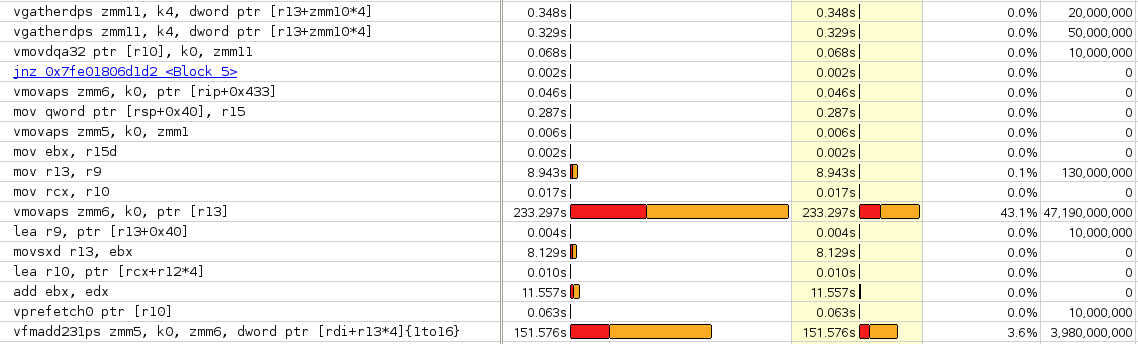
\includegraphics[width=0.9\textwidth]{figures/vtune_rows.png}
    \caption{Vtune analysis assembly code generated for the Xeon Phi.}
    \label{vtune_rows}
\end{figure}


\par{This kernel for Intel Xeon Phi and Xeon achieved a performance improvement in comparison with previous kernels as it can 
    be seen in figure \ref{Rows}. The use of OpenCL \emph{private memory} immediatelly increment the L1 hit ratio in both Intel
    Architectures(Xeon and Xeon Phi), also increments the vectorization intensity. Also we can see the effect of lost of parallelism
    due to the small amount of \emph{work groups} scheduled after a \emph{work group} of dimension of 128.}

\begin{figure}[!h]
    \centering
    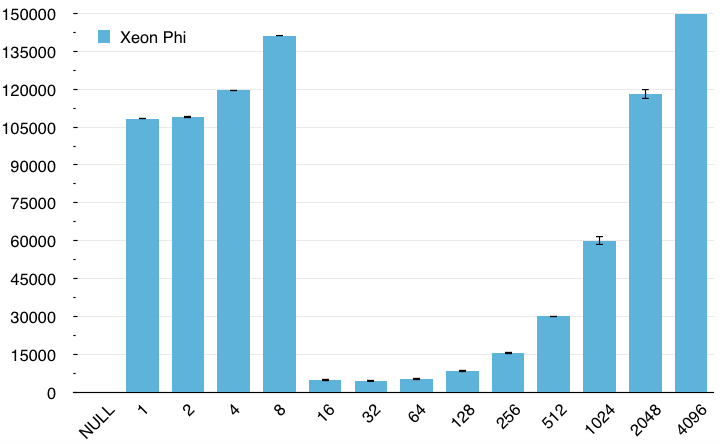
\includegraphics[width=0.49\textwidth]{figures/opt2_phi.png}
    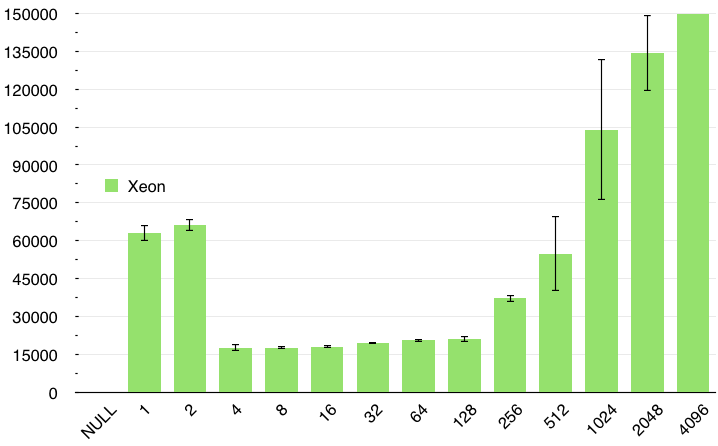
\includegraphics[width=0.49\textwidth]{figures/opt2_cpu.png}
    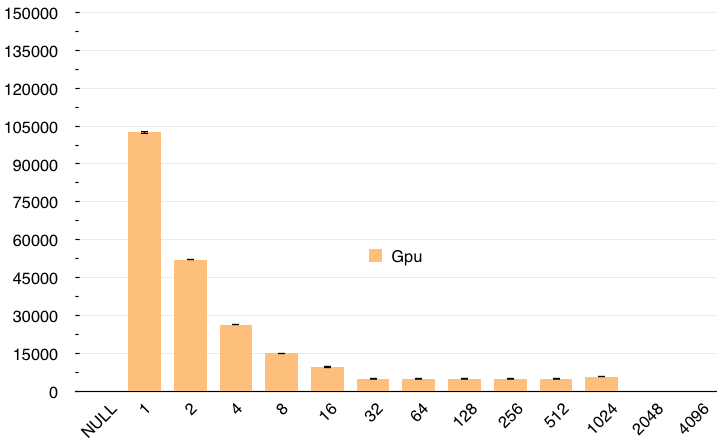
\includegraphics[width=0.49\textwidth]{figures/opt2_gpu.png}
    \caption{Row optimisation matrix multiplication in different architectures.}
    \label{Rows}
\end{figure}


\par{In this case the most performant architecture for this kernel is the Intel Xeon Phi as it can be seen \ref{RowsComp}, 
    showing how sensible the Intel Xeon Phi in terms of memory optimisations.(\emph{more on this, other perspective of the plot})}


